\par Como se mencionó anteriormente, el objetivo de esta etapa es explorar distintas mecánicas y conceptos de juego, para luego definir el \textit{vertical slice} y los \textit{project goals}. En base a esto se divide el proceso en 2 etapas; una de prototipado, donde se prueban varias ideas, y otra de iteración y creación de un \textit{vertical slice}, donde se trabaja sobre el prototipo más llamativo.
%
%
\subsection{Prototipado}
\subsubsection{Prototipo 1}
\par Siguiendo el consejo de Anderson, el primer prototipo se realizó en el marco de la \textit{GMTK Jam} \cite{GMTKGameJam}, llevada a cabo del 30 de julio al 3 de agosto de 2025 y cuyo tema fue el concepto de \textit{loop}.
\par En base a la idea se comenzó un juego del género \textit{endless runner}, donde el jugador recorre un mapa infinito realizando acciones como saltar parae esquivar obstáculos hasta perder. Un ejemplo de este tipo de juegos es \textit{Chrome Dino}, el cual aparece en el navegador Chrome cuando no hay conexión a internet. En este juego, el jugador controla un dinosaurio que corre por un desierto, saltando sobre cactus y esquivando pájaros hasta chocar con alguno de ellos \cite{DinosaurGame2025}.
\begin{figure}[H]
  \centering
  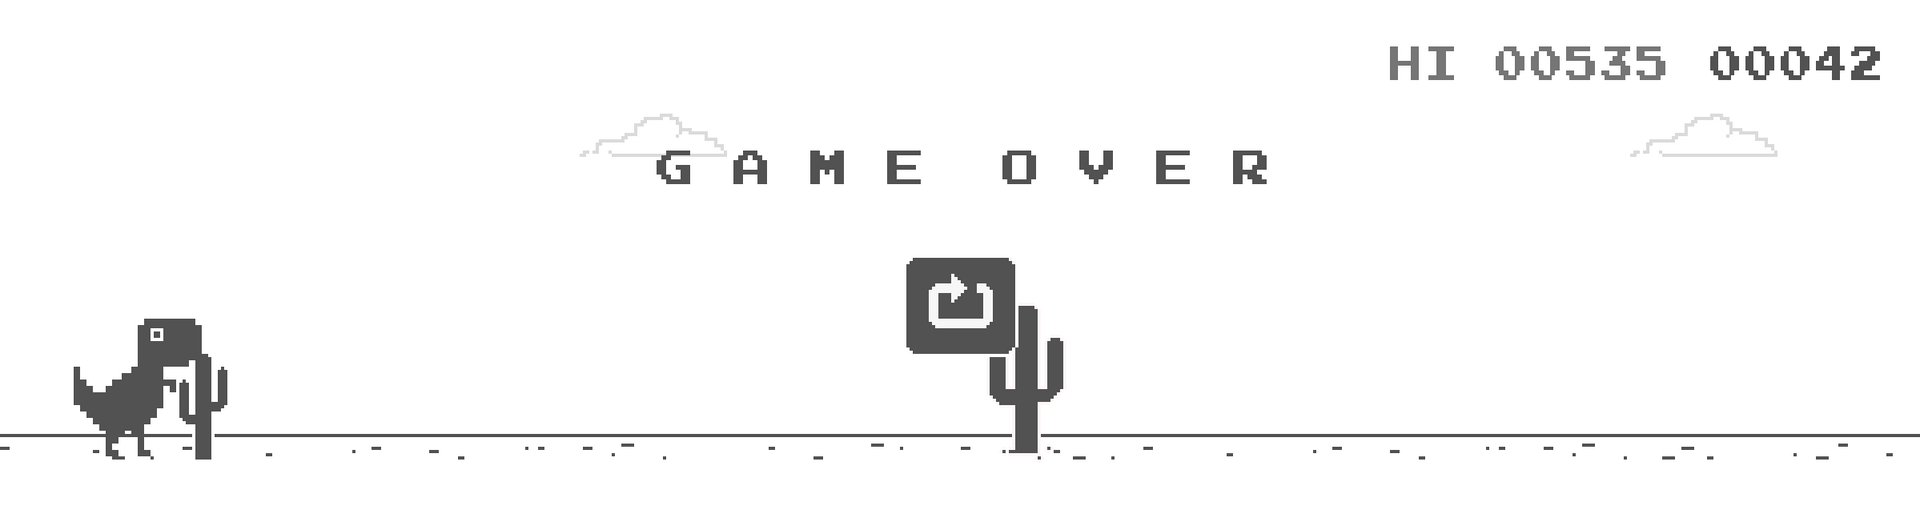
\includegraphics[width=\textwidth]{dinosaur_game.png}
  \caption{Captura de pantalla de \textit{Dinosaur Game}. Extraída de \cite{DinosaurGame2025}.}
  \label{fig:x dinosaur game} 
\end{figure}
\par Siguiendo este concepto, se comenzó con un prototipo donde el jugador personifica a un skater que esquiva obstáculos mientras derrapa sobre una barandilla en forma de loop. El objetivo del juego es recorrer la mayor distancia posible, mientras se esquivan obstáculos y se realizan trucos para sumar puntos.
\begin{figure}[H]
  \centering
  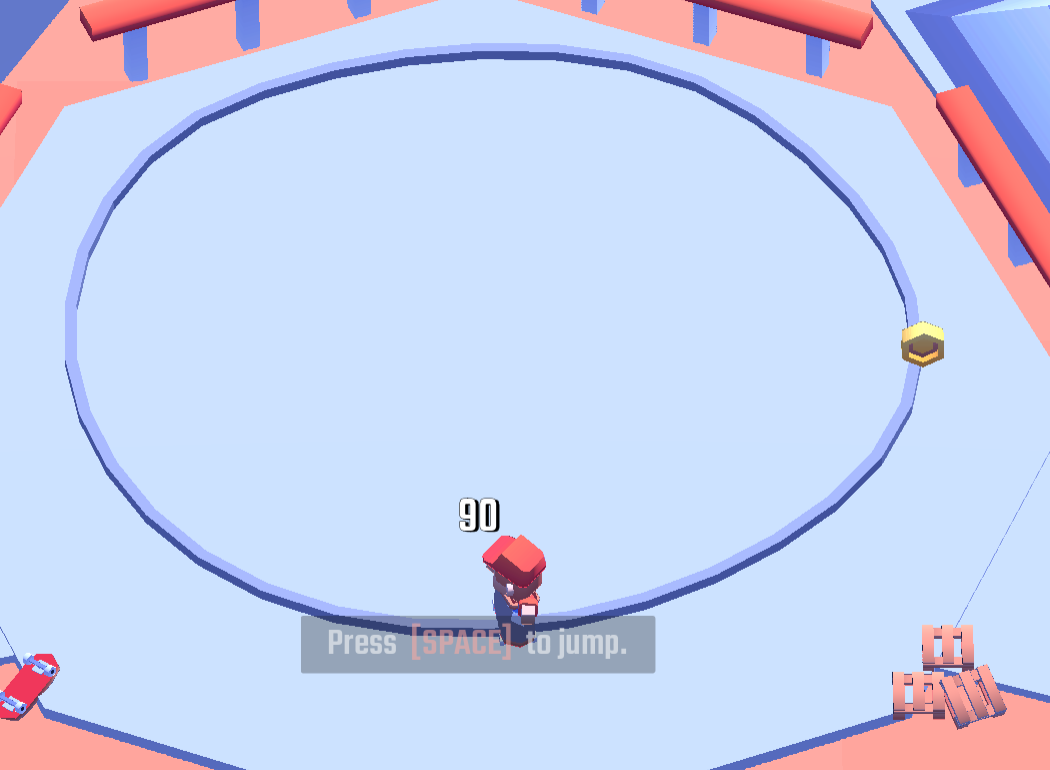
\includegraphics[width=\textwidth]{grind_the_grind_1.png}
  \caption{Captura de pantalla del prototipo. El jugador derrapa sobre una barandilla en forma de loop. Creada por autor.}
  \label{fig:x grind the grind 1} 
\end{figure}
\par Sin embargo, se encontraron dificultades para implementar el concepto. Si bien la acción de derrapar y realizar trucos era interesante, los obstáculos no aportaban diversión al juego. Debido a esto se decidió virar el concepto a un juego del género \textit{incremental}, donde el jugador debe derrapar y realizar trucos para sumar puntos y mejorar su skater. Los juegos incrementales se enfocan en recolectar recursos de forma pasiva para mejorar al jugador y y optimizar aún mas dicha obtención de recursos.
\par En este caso, el objetivo del juego es obtener la mayor cantidad de puntos posibles, los cuales se consiguen realizando trucos y derrapando. Cada cierta cantidad de puntos, además de recolectando monedas, se otorga dinero al jugador que puede utilizar para mejorar el proceso. El juego presenta 3 mejoras:
\begin{itemize}
    \item \textbf{Trucos}: Aumenta la cantidad de puntos obtenidos por cada truco realizado.
    \item \textbf{Derrape}: Aumenta la cantidad de puntos obtenidos por derrapar.
    \item \textbf{Velocidad}: Aumenta la velocidad en la que se obtienen puntos al derrapar.
\end{itemize}
\begin{figure}[H]
  \centering
  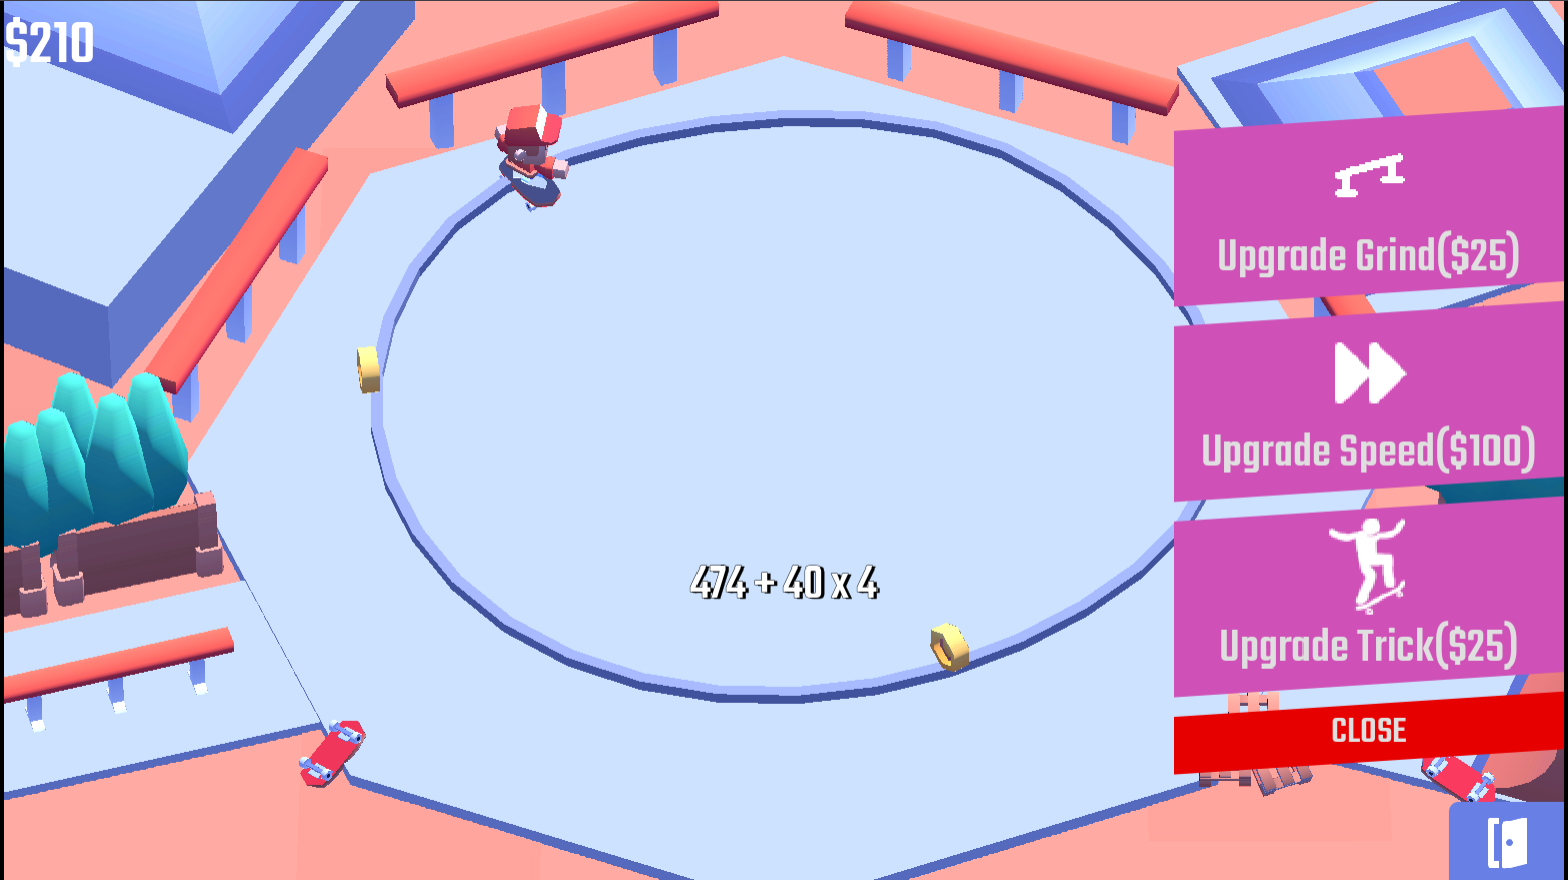
\includegraphics[width=\textwidth]{grind_the_grind_2.png}
  \caption{Captura de pantalla del segundo prototipo. El jugador obtiene puntos al realizar acciones, y recibe dinero para comprar mejoras. Creada por autor.}
  \label{fig:x grind the grind 2} 
\end{figure}
\par En el aspecto técnico, juego se desarrolló con el motor gráfico \textit{Godot} para la plataforma web y Windows. El arte y sonido se obtuvo mayormente de internet, utilizando recursos libres de derechos de autor. En particular, se utilizó arte de \textit{Kenney.nl} \cite{kenneyHomeKenney} y \textit{OpenGameArt} \cite{OpenGameArtorg}, y música de \textit{Free Music Archive} \cite{RoyaltyFreeMusic}.
\begin{figure}[H]
  \centering
  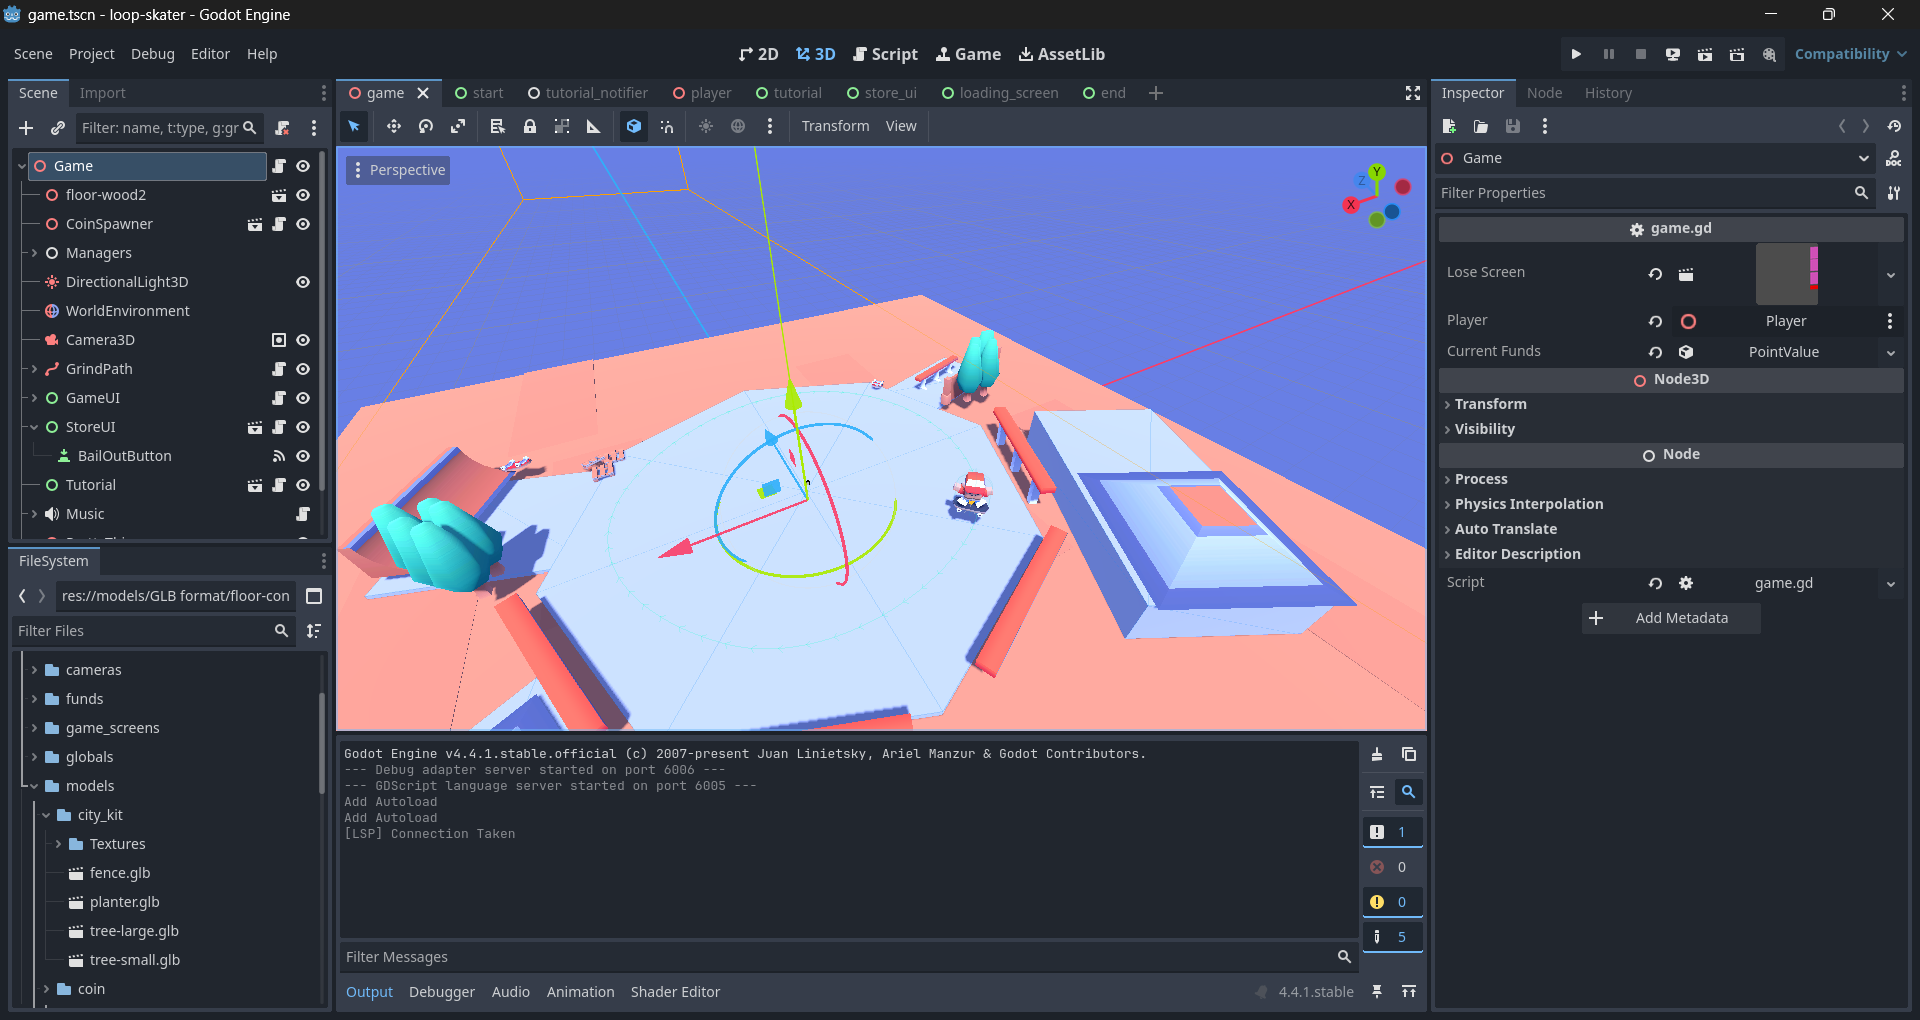
\includegraphics[width=\textwidth]{godot_1.png}
  \caption{Captura de pantalla del proyecto en Godot. Creada por autor.}
  \label{fig:x godot 1} 
\end{figure}

\par Una ventaja del evento en el que se participó es que al finalizar el periodo de desarrollo, los jugadores estaban invitados a calificar los juegos en distintas categorias: creatividad, diversión, narrativa, arte y sonido. Cada participante recibía una lista de juegos aleatorios para evaluar.
\par En general, el juego recibió críticas mixtas. Algunos jugadores apreciarion el aspecto visual y sonoro del juego, pero también remarcaron que la progresión del mismo era demasiado rápida \cite{GrindGrindFollowtherules}.
\begin{figure}[H]
  \centering
  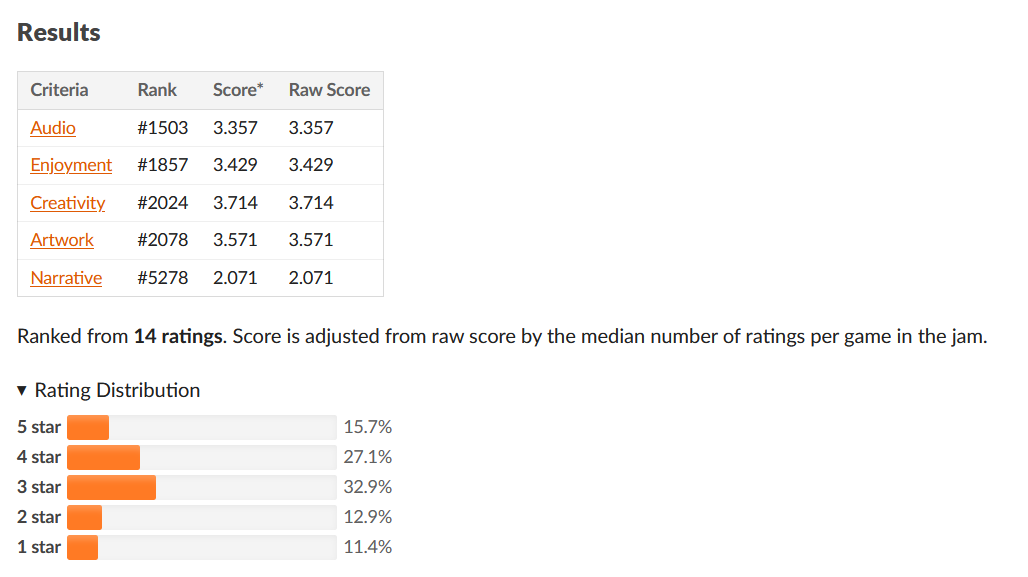
\includegraphics[width=\textwidth]{prototype_1_ratings.png}
  \caption{Calificaciones del juego presentado. Captura obtenida de \cite{GrindGrindFollowtherules}.}
  \label{fig:x calificaciones prototipo 1} 
\end{figure}
\par Al finalizar el periodo de votación, se lanzó una actualización arreglando los problemas de progresión encontrados. \todo{tengo las builds en una carpeta de drive. Como lo indico?} %TODO: tengo las builds en una carpeta de drive. Como lo indico? 
%
%
\subsubsection{Prototipo 2}
\par Para el segundo prototipo se volvió a participar en una \textit{game jam}, esta vez en la \textit{Godot Wild Jam 84} \cite{GodotWildJam}, realizada del 8 de agosto al 17 de agosto de 2025. En este evento, el tema a cumplir fue \textit{critters} (bicho o animal pequeño en español).
\par El proyecto se comenzó creando un  \textit{\hyperref[sec:ideation_lemarchand]{mind map}}, comenzando por la idea de \textit{critters} y expandiendolo en distintos conceptos relacionados.
%
\begin{figure}[H]
  \centering
  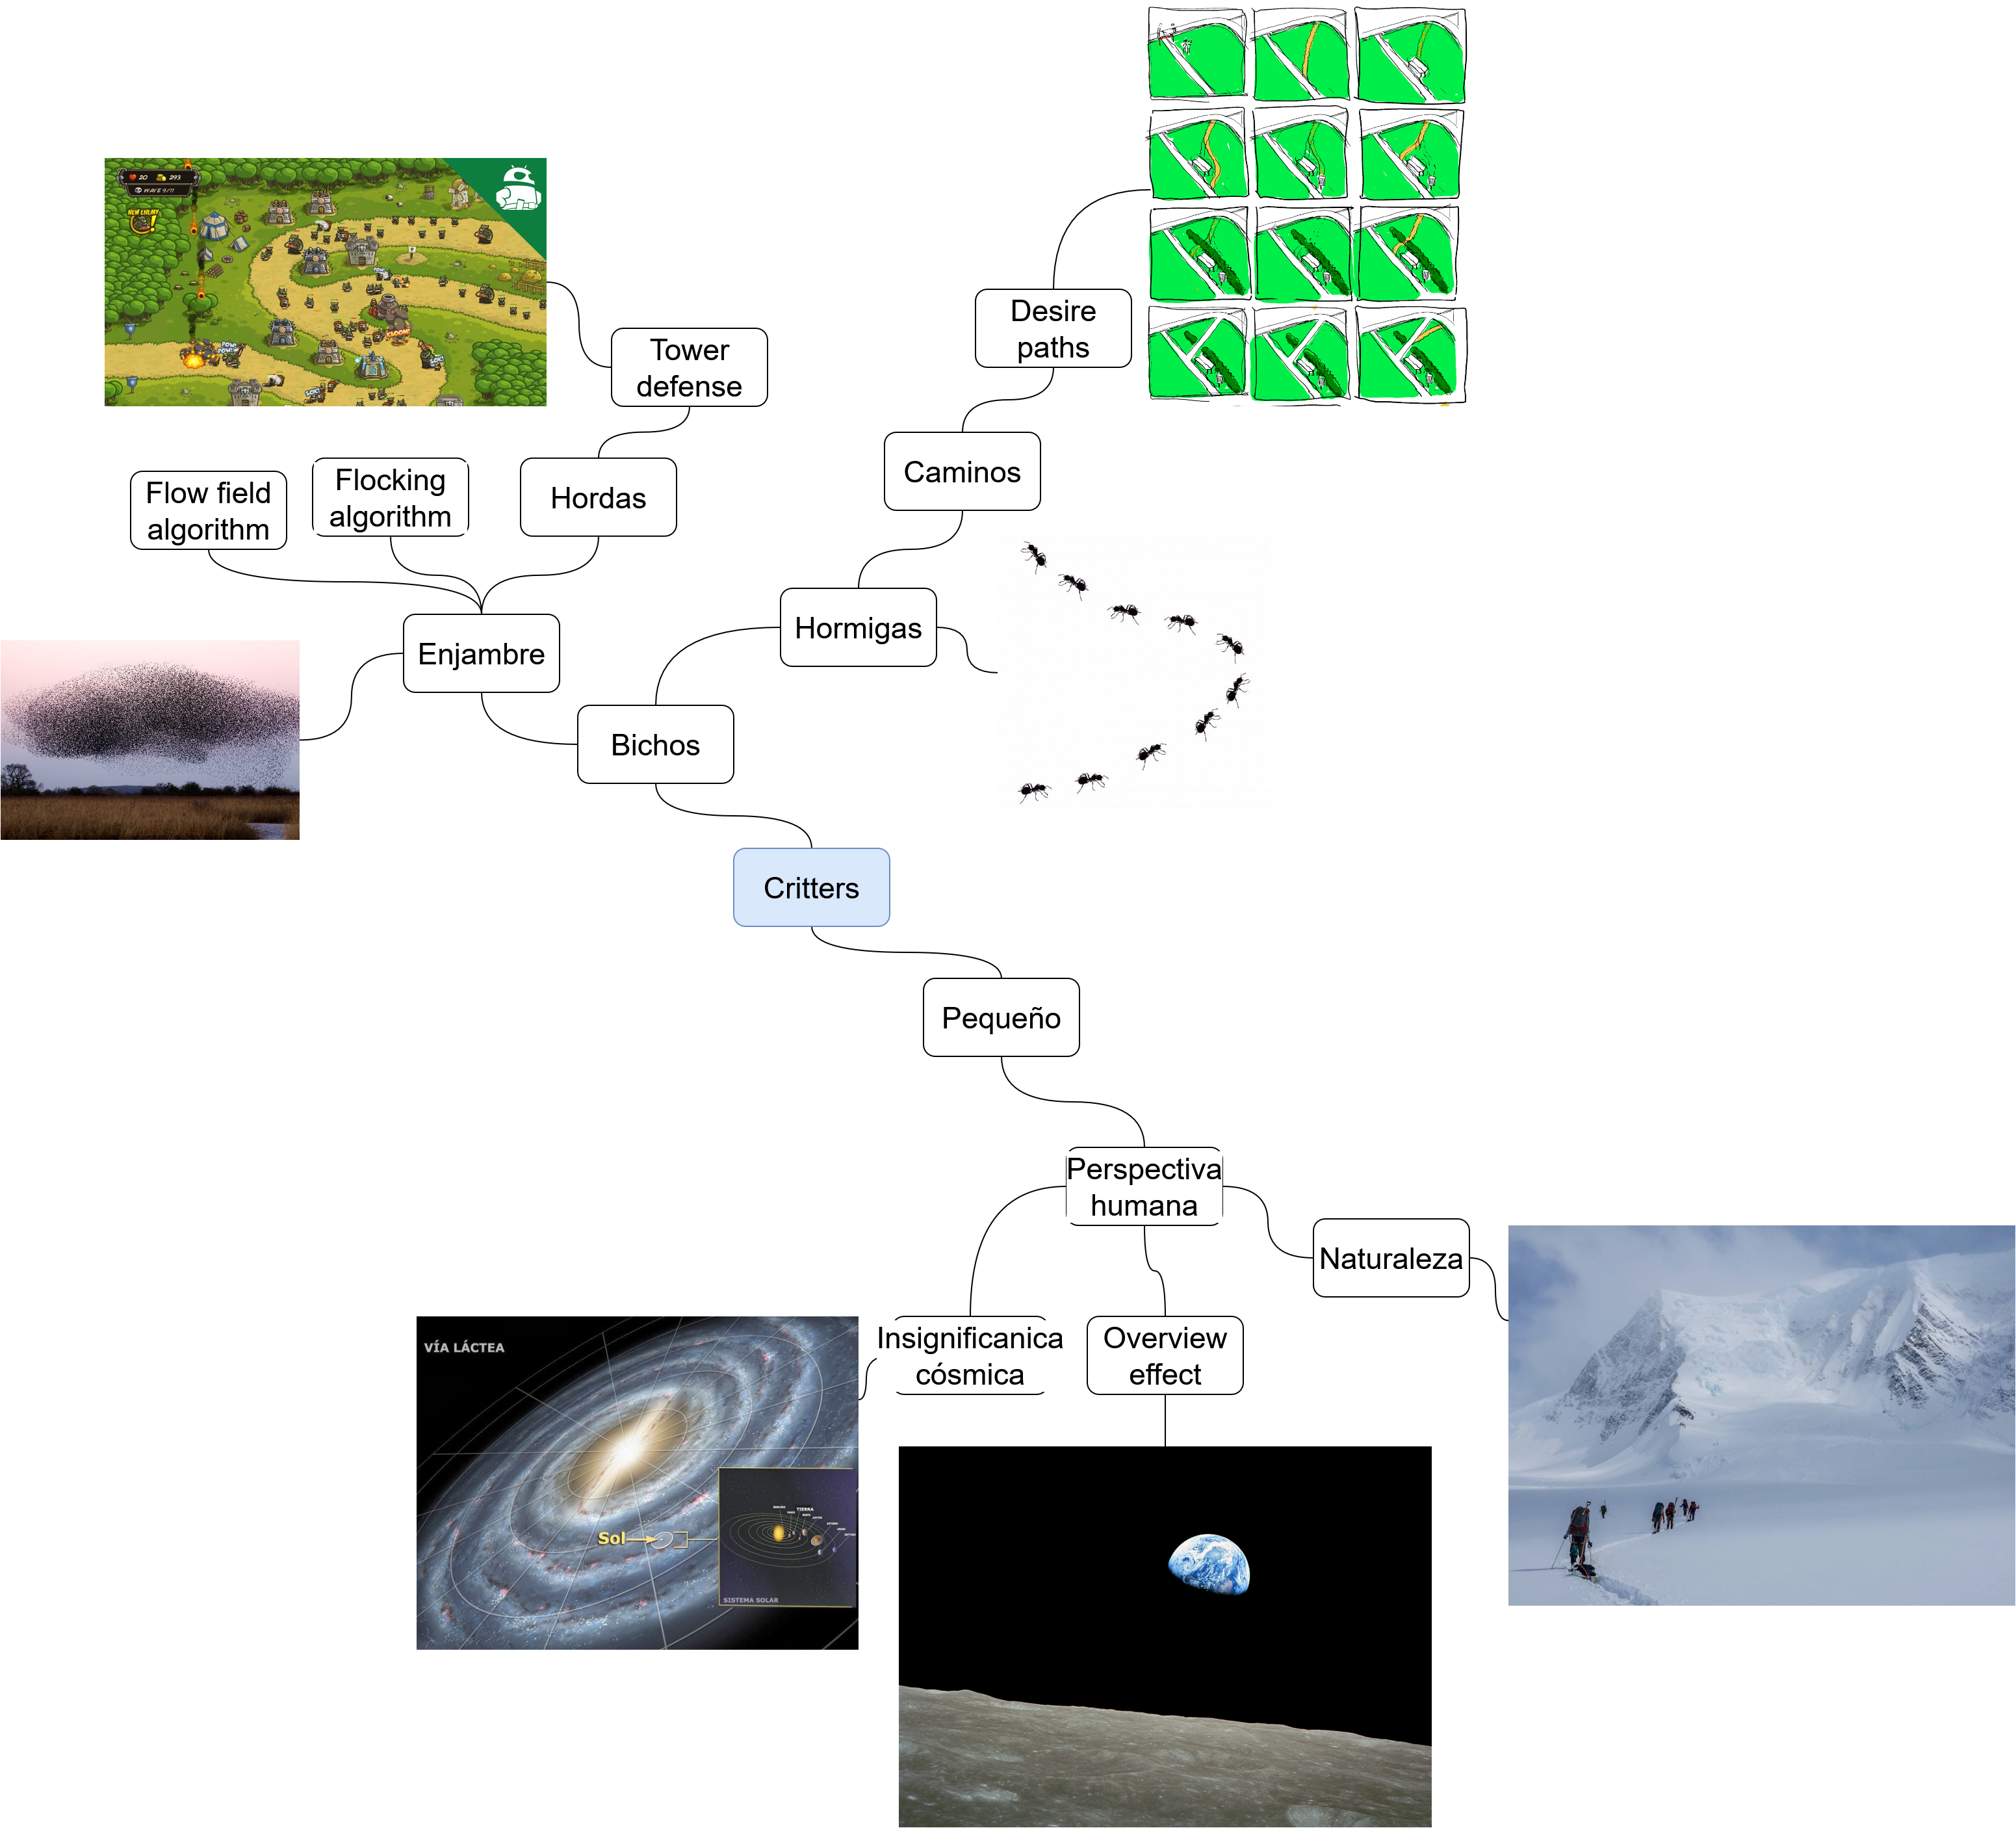
\includegraphics[width=\textwidth]{prototype_2_mindmap.png}
  \caption{\textit{Mind map} creado en base al concepto de \textit{critters}. Creada por autor.}
  \label{fig:x mindmap prototipo 2} 
\end{figure}
\par En base a esta exploración de ideas, se decidió realizar un juego donde el jugador controla una horda de goblins, los cuales deben eliminar enemigos para sumar compañeros a la horda y obtener mejoras.
\par El proyecto estaba inspirado en el juego \textit{Vampire Survivors}, donde el jugador debe sobrevivir oleadas de enemigos que atacan al jugador constantemente. Por cada enemigo eliminado, el jugador recibe puntos de experiencia que puede utilizar para obtener mejoras e items y prolonguen su supervivencia.
%
\begin{figure}[H]
  \centering
  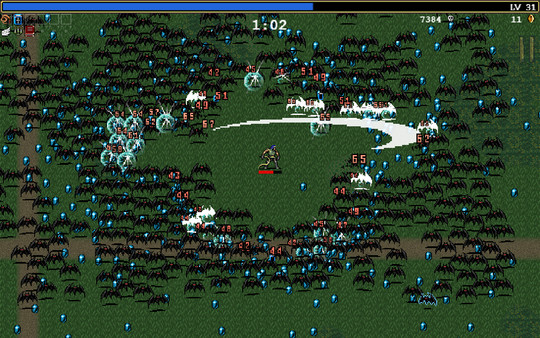
\includegraphics[width=\textwidth]{vampire_survivors.png}
  \caption{Captura de pantalla del videojuego \textit{Vampire Survivors}. Obtenida de \cite{VampireSurvivorsSteam}.}
  \label{fig:x Vampire Survivors} 
\end{figure}
%
\par Un aspecto importante del prototipo era utilizar un tipo de algoritmo llamado \textit{steering behaviors}. El objetivo de este algoritmo es crear entidades dentro de un juego que se mueven de forma autónoma, utilizando información limitada sobre su entorno para cumplir una serie de objetivos. En particular, para formar un comportamiento de horda, las entidades tienen como objetivo llegar a cierta posición mientras tratan de evitar a otras entidades que tienen a su alrededor. Dentro del juego estos comportamientos se modelan utilizando fuerzas, las cuales mueven a los goblins en distintas direcciones de forma que se cumplan los objetivos establecidos \cite{5AutonomousAgentsa,SteeringBehaviorsAutonomous}.
\par En la figura \ref{fig:x seek repel forces} se puede observar un ejemplo de estas fuerzas. \textit{Seek force} empuja al goblin en la dirección de una posición objetivo, mientras que \textit{repel force} lo aleja de otro goblin. Estas fuerzas afectan la velocidad de la entidad, cambiando el rumbo del personaje.
%
\begin{figure}[H]
  \centering
  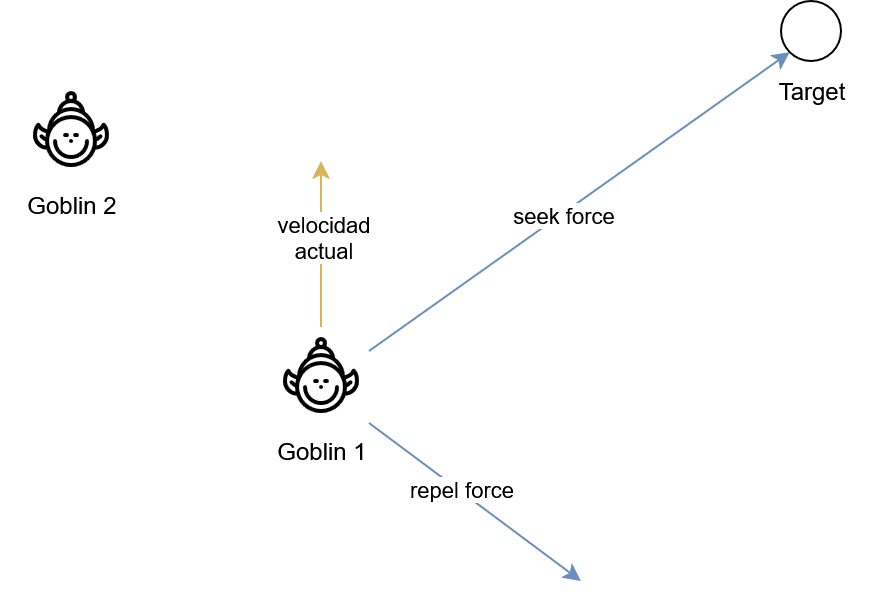
\includegraphics[width=\textwidth]{seek_repel_example.png}
  \caption{Ejemplo de las fuerzas que afectan a una entidad en un algoritmo de \textit{steering behaviors}. Creada por autor.}
  \label{fig:x seek repel forces} 
\end{figure}
%
\bigbreak
\par Desafortunadamente, el prototipo presentó varias dificultades. En un principio, desarrollar el algoritmo mencionado anteriormente tomó entre 3 y 4 días. Idealmente, la mecánica principal se desarolla lo antes posible, de forma que se pueda validar si realmente es divertida o no. 
\par Una vez se tuvo este sistema, se encontraron dificultades para generar enemigos que complementaran la mecánica principal. El mayor problema surgió de que se decidió que tanto los goblins como los enemigos recibieran daño al chocar entre ellos.
\par Si bien el prototipo es jugable, se decidió no presentarlo en el evento. Se consideró que el juego no estaba en estado de ser probado, y que la mecánicas no eran lo suficientemente divertidas.
%
\begin{figure}[H]
  \centering
  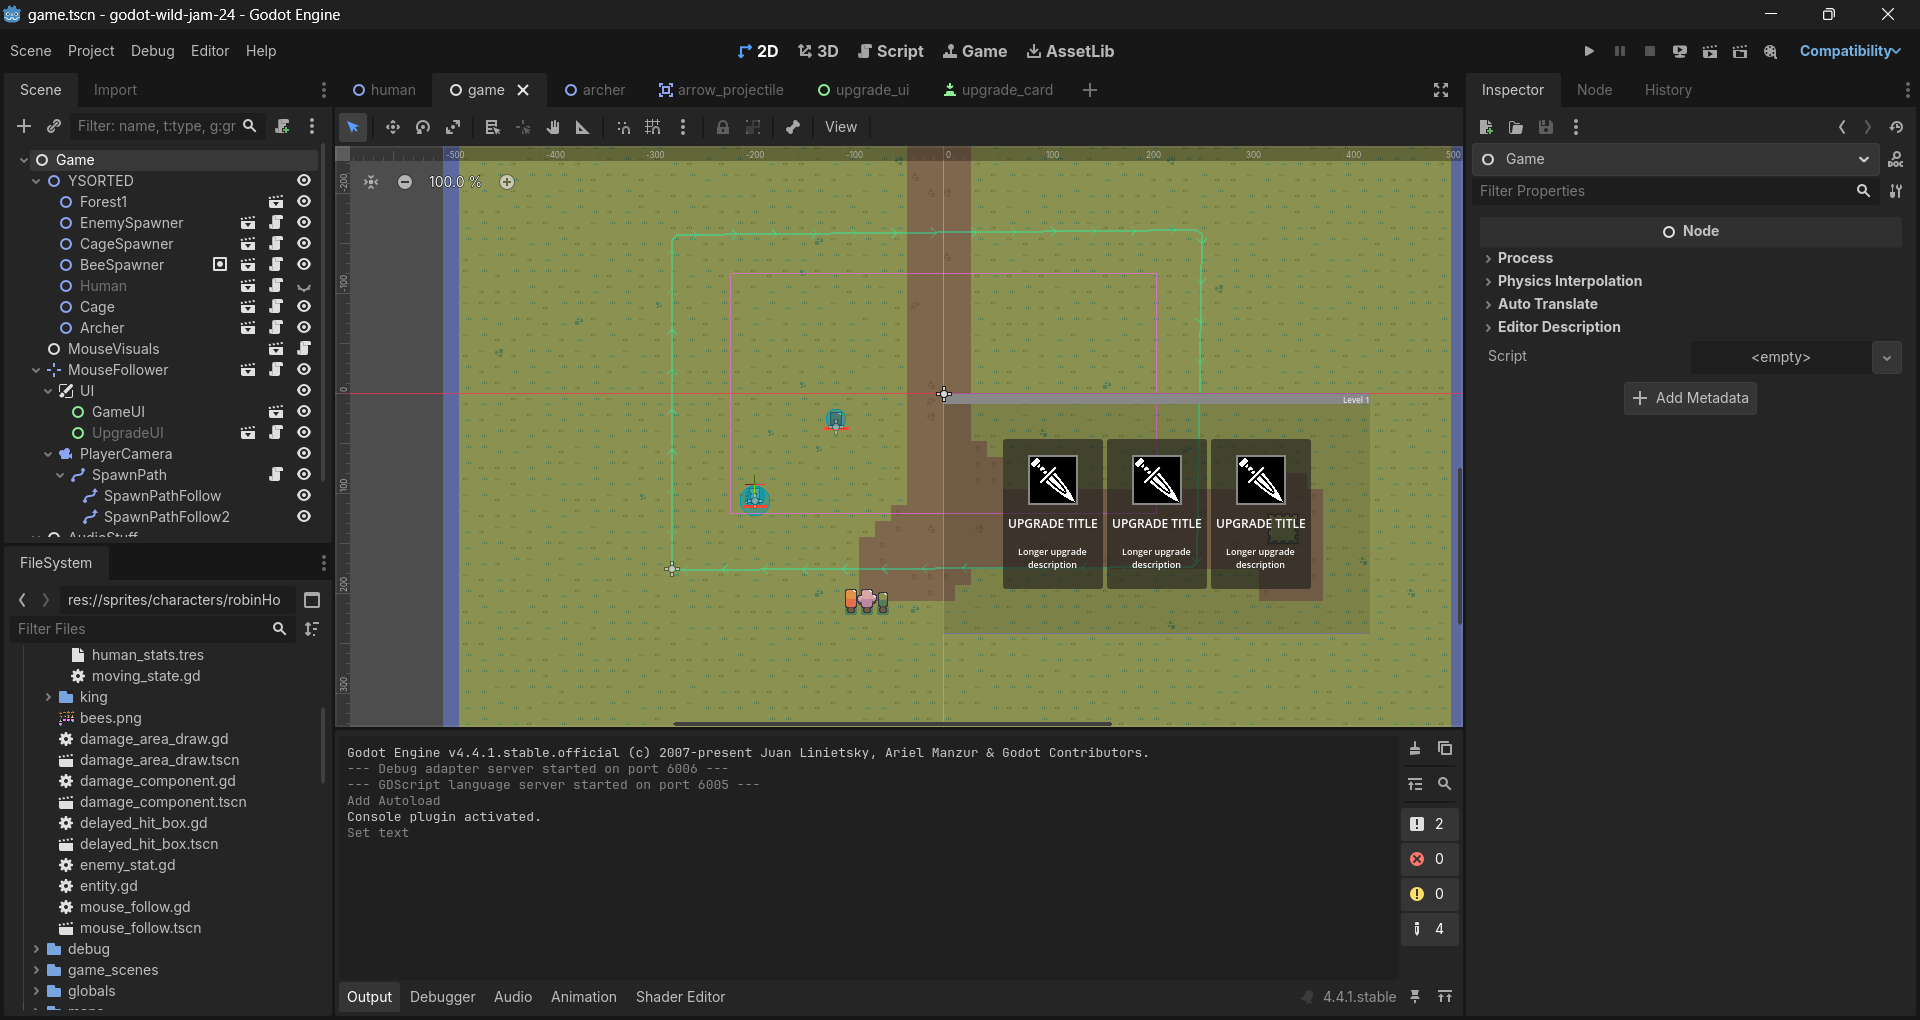
\includegraphics[width=\textwidth]{prototype_2_screenshot.png}
  \caption{Captura de pantalla del segundo prototipo. Creada por autor.}
  \label{fig:x prototipo 2 godot} 
\end{figure}
%
\subsubsection{Prototipo 3}
El tercer prototipo se desarrolló para la \textit{Mega Jam de Invierno}, una jam de 3 días llevada a cabo en Mendoza \cite{MEGAJAMInvierno}. Como otras jams, el evento requería que el juego cumpliera con un temática, en este caso \textit{agua}.
Debido al límite de tiempo, se decidió desarrollar una novela visual. Este tipo de juegos consiste mayormente en situaciones descriptas mediante texto, generalmente acompañadas por imagenes, donde el jugador puede realizar acciones como interactuar con objetos o moverse en el espacio. Además, estas obras suelen tener un fuerte énfasis en la historia y narrativa \cite{VisualNovel2025}.
%
\begin{figure}[H]
  \centering
  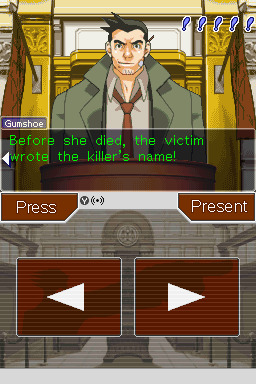
\includegraphics[width=\textwidth]{ace_attorney.png}
  \caption{Captura de pantalla \textit{Ace Attorney}, una serie de novelas visuales popular. Extraída de \cite{FilePhoenixWright2020}.}
  \label{fig:x ejemplo novela visual} 
\end{figure}
%
\par Utilizando la temática establecida, se decidió crear un juego de terror donde el jugador explora un laberinto submarino. El jugador puede moverse entre habitaciones e interactuar con objetos, pero algunas acciones (como la de pasar a una nueva habitación) consumen el limitado oxígeno disponible. El jugador pierde al quedarse sin aire, y gana si encuentra la salida.
%
\begin{figure}[H]
  \centering
  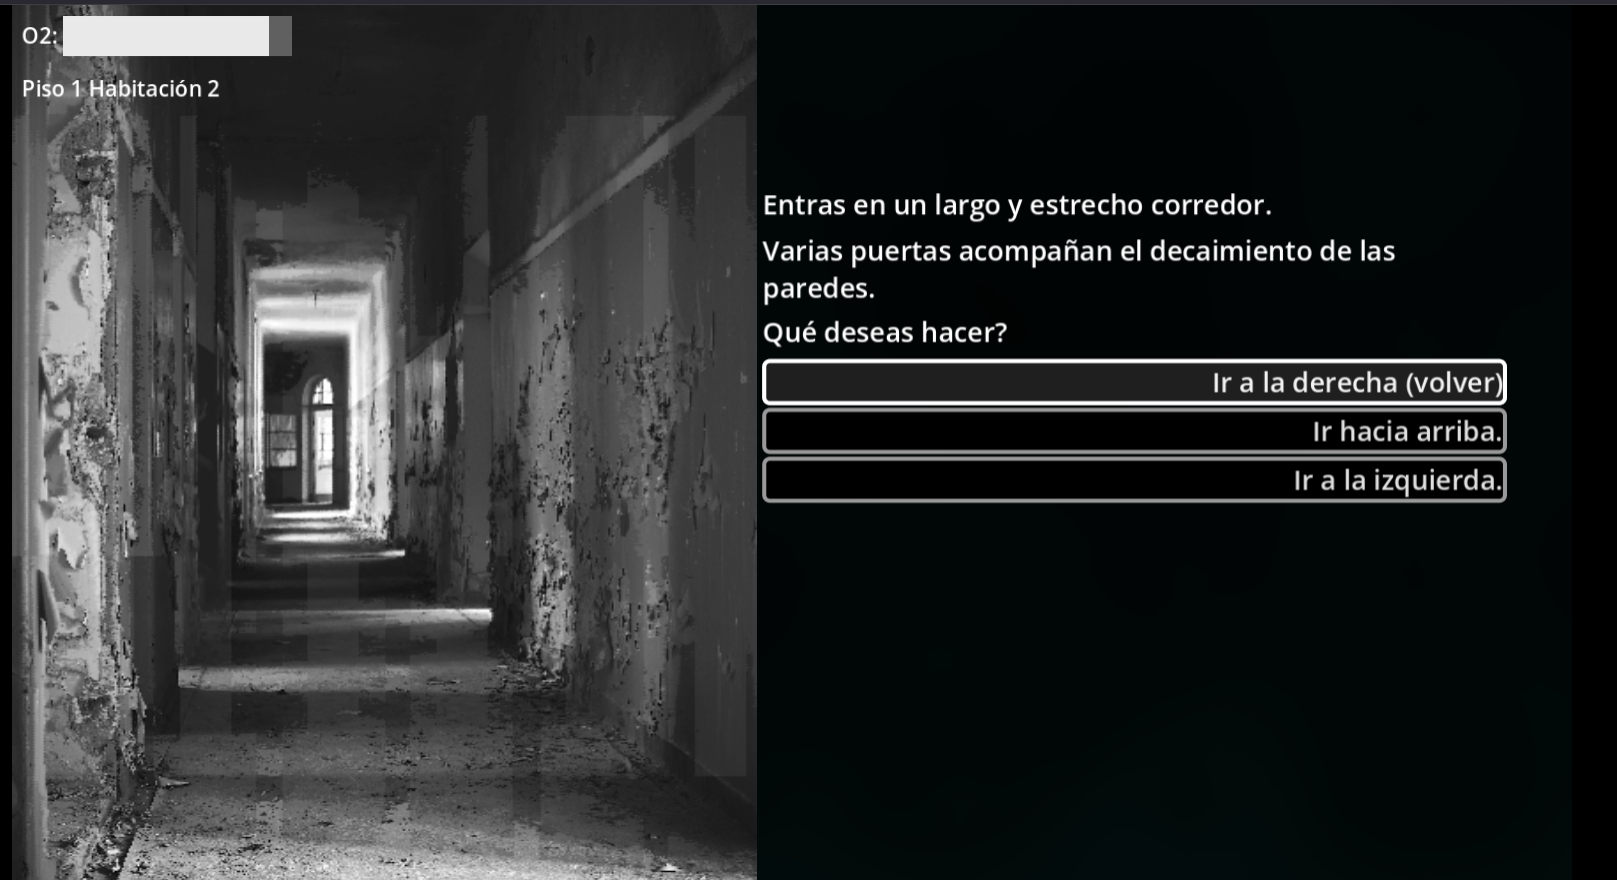
\includegraphics[width=\textwidth]{prototype_3.png}
  \caption{Captura de pantalla del juego desarrollado. Creada por autor.}
  \label{fig:x prototypo 3 captura} 
\end{figure}
%
\par El juego se desarrolló en Godot utilizando un plugin llamado \textit{Dialogue Manager}, el cual proporciona una serie de herramientas que facilitan la creación de un juego narrativo. Para la música, se utilizaron \textit{asset packs} de itch.io. Para el arte, se usaron imágenes de sitios como Pexels, Freepik y Pixabay \cite{57MillionStunning,FreepikAllinOneAI,FotosStockGratis}, las cuales están libres de derechos de autor.
\bigbreak
\par A diferencia de otras jams, en esta no hubo una etapa de feedback. Debido a esto, se decidió compartir el juego en grupos de desarrolladores. En general, el juego recibió críticas positivas, destacando la narrativa y la inmersión presentada al jugar.